\chapter{BSM signatures in di-tau final states}


\section{A Simplified Model for the $\tilde S_1$ Scalar Leptoquark}

Leptoquarks (LQs) are hypothetical bosonic particles that couple simultaneously to a quark and a lepton, thereby mediating lepton-quark interactions at a single vertex. They arise naturally in various extensions of SM, including grand unified theories and models with extended gauge symmetries, and have attracted renewed interest as a possible explanation for observed flavor anomalies and hints of lepton flavor non-universality.

To ensure Lorentz invariance, the interaction vertex involving a leptoquark, a quark, and a lepton must form a scalar or vector operator. Among these possibilities, scalar leptoquarks (scalar-LQs) provide a minimal and renormalizable framework without requiring new gauge interactions, making them an ideal starting point for simplified model studies.

The classification of scalar leptoquarks is determined by their transformation properties under the SM gauge group $SU(3)_C \times SU(2)_L \times U(1)_Y$. For simplicity, we focus on scalar-LQs that are singlets under $SU(2)_L$, so that the model contains a single new scalar degree of freedom. This constraint leads to interactions involving two fermions of the same chirality, which requires charge conjugation of one of the fields to build a Lorentz scalar.

There are two classes of gauge-invariant, renormalizable operators that couple such a singlet scalar-LQ to SM fermions. These are:

\begin{enumerate}
    \item $I_1 = \overline{q}_L^C \vb*{\epsilon} \ell_L$ and $I_1' = \overline{u}_R^C e_R$, where $q_L$ and $\ell_L$ are left-handed quark and lepton doublets, respectively, and $u_R$, $e_R$ are right-handed singlets. Both $I_1$ and $I_1'$ are $SU(2)_L$ singlets, transform as color triplets under $SU(3)_C$, and carry hypercharge $Y = -2/3$.
    \item $\tilde I_1 = \overline{d}_R^C e_R$, a gauge-invariant operator involving two right-handed singlets. It is also a color triplet and an $SU(2)_L$ singlet, but with hypercharge $Y = -8/3$.
\end{enumerate}

The corresponding leptoquark representations are:
\begin{enumerate}
    \item $S_1 \dot= (\bar{\mathbf{3}}, \mathbf{1}, 2/3)$, consistent with the first set of operators.
    \item $\tilde{S}_1 \dot= (\bar{\mathbf{3}}, \mathbf{1}, 8/3)$, associated with the second invariant.
\end{enumerate}

In models with flavor alignment or preferential couplings to third-generation fermions, $S_1$ typically couples to $b\nu_\tau$ and $t\tau$ vertices. However, processes like $pp \to \tau^+\tau^-$ suffer suppression due to the low parton density of the top quark in the proton. 

In contrast, the $\tilde{S}_1$ leptoquark allows for direct couplings to $b$ quarks and $\tau$ leptons via a term of the form $\overline{d}_R^C \tilde{S}_1 e_R$. Despite the relatively small $b$-quark content in the proton, these channels remain accessible at the LHC.

For these reasons, this section focuses on the simplified model containing only the scalar leptoquark $\tilde{S}_1$. The most general renormalizable Lagrangian for the $\tilde{S}_1$ leptoquark extends the SM one by
\begin{equation}
    \mathcal{L}\supset |D_\mu\tilde{S}_1|^2 + \tilde{y}_{ij} \overline{d}_R^{C\,i} \tilde{S}_1 e_R^j + \tilde{z}_{ij} \overline{u}_R^{C\,i} \tilde{S}_1^* u_R^j + \text{h.c.} + V_{\text{ext}}(\tilde{S}_1,H)
\end{equation}
where $\vb*{\tilde{y}}, \vb*{\tilde{z}}$ are complex Yukawa matrices in the flavor space\marginpar{Note that $\vb*{\tilde{z}}$ must be antisymmetric (due to fermionic statistics) and is typically assumed to vanish or be highly suppressed to avoid large FCNCs.}, $D_\mu$ is the covariant derivative acting on the $\tilde{S}_1$ field as 
\begin{equation}
    D_\mu \tilde{S}_1 = \partial_\mu \tilde{S}_1 + i g_s T^a G_\mu^a \tilde{S}_1 + i \frac{4}{3} g' B_\mu \tilde{S}_1,
\end{equation}
and $V_{\text{ext}}$ is the extension of the SM Higgs potential to include the leptoquark field gived by
\begin{equation}
    V_{\text{ext}} = \mu_{\tilde{S}_1}^2 |\tilde{S}_1|^2 + \lambda_{\tilde{S}_1} |\tilde{S}_1|^4 + \lambda_{H\tilde{S}_1} |H|^2 |\tilde{S}_1|^2,
\end{equation}
such that the full scalar potential reads
\begin{equation}
    V = \underbrace{-\mu^2|H|^2 + \lambda|H|^4}_{\text{SM Higgs}} + \underbrace{\mu_{\tilde{S}_1}^2|\tilde{S}_1|^2 + \lambda_{\tilde{S}_1}|\tilde{S}_1|^4}_{\text{scalar-LQ self-interactions}} + \underbrace{\lambda_{H\tilde{S}_1}|H|^2|\tilde{S}_1|^2}_{\text{Higgs portal}}.
\end{equation}

After EWSB, $H \to (0, (v+h)/\sqrt{2})^T$, the $H\tilde S_1$ interactions become in interactions between the physical Higgs boson $h$ and the leptoquark $\tilde{S}_1$ as
\begin{align}
    \mathcal{L}_{\text{int}} &\supset \lambda_{H\tilde{S}_1}v h|\tilde{S}_1|^2 + \frac{1}{2}\lambda_{H\tilde{S}_1}h^2|\tilde{S}_1|^2
\end{align}
and a mass shift for the leptoquark field
\begin{equation}
    \Delta m_{\tilde{S}_1}^2 = \frac{1}{2}\lambda_{H\tilde{S}_1}v^2 \implies m_{\tilde{S}_1}^2 = \mu_{\tilde{S}_1}^2 + \frac{1}{2}\lambda_{H\tilde{S}_1}v^2.
\end{equation}
Additionally, from the covariant derivative as $B_\mu = c_W A_\mu - s_W Z_\mu$, the $\tilde{S}_1$ interactions with the SM gauge bosons are given by
\begin{align}
    \mathcal{L} &\supset \frac{4}{3}e\left[(\partial_\mu\tilde{S}_1^*)\tilde{S}_1 - \tilde{S}_1^*(\partial_\mu\tilde{S}_1)\right]A^\mu + \left(\frac{4}{3}e\right)^2 A_\mu A^\mu |\tilde{S}_1|^2\\
    \mathcal{L} &\supset -\frac{4}{3}g_1 s_W\left[(\partial_\mu\tilde{S}_1^*)\tilde{S}_1 - \tilde{S}_1^*(\partial_\mu\tilde{S}_1)\right]Z^\mu + \left(\frac{4}{3}g_1 s_W\right)^2 Z_\mu Z^\mu |\tilde{S}_1|^2.
\end{align}

For preferential couplings to third-generation fermions in the lepton-quark vertices, we assume the texture of the Yukawa matrix $\tilde{y}_{33}$ is such that $\tilde{y}_{33} \gg \tilde{y}_{ij}$ for $i,j \neq 3$. This results in a preferential decay of the scalar-LQ into $b\tau$ final states, with branching ratio ${\rm BR}(\tilde{S}_1 \to b\tau) \approx 1$ for large scalar-LQ masses. 

\begin{center}
    \includegraphics[width=.9\linewidth]{Images/sLQ_Cross_Section.pdf}
    \captionof{figure}{Cross section for scalar leptoquark (scalar-LQ) pair production decaying to $\tau^+\tau^-$ final states, showing different $\tau$ polarization configurations as a function of scalar-LQ mass at $\sqrt{s}=13.0\; \si{\tera\electronvolt}$. The coupling is fixed to  $\tilde{y}_{33} = 1.0$.}\label{fig:cross_section_scalar-LQ}
\end{center}

It is worth noting that, due to the right-handed structure of the Yukawa interaction the scalar leptoquark $\tilde{S}_1$ couples only to right-chiral tau leptons. As a result, the dominant contribution to the $\tau^+\tau^-$ final state originates from the configuration where the outgoing taus have opposite helicities, specifically $\tau^+_L \tau^-_R$. This polarization asymmetry provides a characteristic signature that could be probed using polarization-sensitive observables, such as the asymmetry in the charged energy of the products of the $\tau$ decay. Figure~\ref{fig:cross_section_scalar-LQ} shows the integrated production cross sections at $\sqrt{s} = 13.0\; \si{\tera\electronvolt}$ assuming a fixed coupling $\tilde{y}_{33} = 1.0$.

% \section{The 2HDM Type-II Model}
% The two-Higgs-doublet model (2HDM) extends the Standard Model (SM) through the addition of a second $SU(2)_L$ Higgs doublet. This extension predicts the existence of three neutral Higgs bosons ($h$, $H$, $A$) along with charged Higgs bosons $H^{\pm}$. While the 2HDM can incorporate CP-violation, its CP-conserving version is often studied, where the neutral Higgs bosons separate into CP-even states ($h$ and $H$) and a CP-odd state ($A$). In general 2HDM scenarios, tree-level flavor-changing neutral currents (FCNC) may occur, but these can be eliminated by implementing a $\mathbb Z_2$ discrete symmetry, leading to different Yukawa coupling structures classified as Type-I, Type-II, lepton-specific (L2HDM), flipped, and inert 2HDM.

% The general scalar potential of 2 HDM is given as
% \begin{equation}
% \begin{aligned}
% V_{\text {tree }}= & m_{11}^2\left(\Phi_1^{\dagger} \Phi_1\right)+m_{22}^2\left(\Phi_2^{\dagger} \Phi_2\right)-m_{12}^2\left(\Phi_1^{\dagger} \Phi_2+\text { h.c. }\right) \\
% & +\frac{\lambda_1}{2}\left(\Phi_1^{\dagger} \Phi_1\right)^2+\frac{\lambda_2}{2}\left(\Phi_2^{\dagger} \Phi_2\right)^2+\lambda_3\left(\Phi_1^{\dagger} \Phi_1\right)\left(\Phi_2^{\dagger} \Phi_2\right)+\lambda_4\left(\Phi_1^{\dagger} \Phi_2\right)\left(\Phi_2^{\dagger} \Phi_1\right) \\
% & +\left[\frac{\lambda_5}{2}\left(\Phi_1^{\dagger} \Phi_2\right)^2+\lambda_6\left(\Phi_1^{\dagger} \Phi_1\right)\left(\Phi_1^{\dagger} \Phi_2\right)+\lambda_7\left(\Phi_2^{\dagger} \Phi_2\right)\left(\Phi_1^{\dagger} \Phi_2\right)+\text { h.c. }\right]
% \end{aligned}    
% \end{equation}
% and the $\Phi_1$ and $\Phi_2$ are complex Higgs doublets with hypercharge $Y=1$ :

% \begin{equation}
% \Phi_1=\binom{\phi_1^{+}}{\frac{1}{\sqrt{2}}\left(v_1+\phi_1+\mathrm{i} a_1\right)}, \quad \Phi_2=\binom{\phi_2^{+}}{\frac{1}{\sqrt{2}}\left(v_2+\phi_2+\mathrm{i} a_2\right)} .    
% \end{equation}
% Here we restrict to the CP-conserving models in which all $\lambda_i$ and $m_{12}^2$ are real and the electroweak vacuum expectation values (VEVs) $v_1$ and $v_2$ are also real with $v^2=v_1^2+v_2^2=$ $(246 \mathrm{GeV})^2$.

% However, because the $\mathbb Z_2$ symmetry, the $\lambda_6$ and $\lambda_7$ terms in the general scalar potential are absent, while the soft breaking $m_{12}^2$ term is still allowed. The mass parameters $m_{11}^2$ and $m_{22}^2$ in the potential are determined by the potential minimization conditions at $\left(v_1, v_2\right)$
% \begin{align}
% m_{11}^2&=m_{12}^2 t_\beta-\frac{1}{2} v^2\left(\lambda_1 c_\beta^2+\lambda_{345} s_\beta^2\right) \\
% m_{22}^2&=m_{12}^2 / t_\beta-\frac{1}{2} v^2\left(\lambda_2 s_\beta^2+\lambda_{345} c_\beta^2\right)
% \end{align}
% where the shorthand notations $t_\beta \equiv \tan \beta=v_2 / v_1, s_\beta \equiv \sin \beta, c_\beta \equiv \cos \beta$, and $\lambda_{345}=$ $\lambda_3+\lambda_4+\lambda_5$ are employed. In this scenario, the vacuum stability requires the following conditions to be satisfied
% \begin{equation}
%     \lambda_1>0, \quad \lambda_2>0, \quad \lambda_3+\sqrt{\lambda_1 \lambda_2}>0, \quad \lambda_3+\lambda_4-\left|\lambda_5\right|+\sqrt{\lambda_1 \lambda_2}>0,
% \end{equation}
% and the unitarity of the scattering process leads that the magnitude of the following combinations of the $\lambda_i$ parameters must be bounded to be less than $8\pi$
% \begin{align}
% a_{ \pm} & =\frac{3}{2}\left(\lambda_1+\lambda_2\right) \pm \sqrt{\frac{9}{4}\left(\lambda_1-\lambda_2\right)^2+\left(2 \lambda_3+\lambda_4\right)^2} \\
% b_{ \pm} & =\frac{1}{2}\left(\lambda_1+\lambda_2\right) \pm \sqrt{\frac{1}{4}\left(\lambda_1-\lambda_2\right)^2+\lambda_4^2} \\
% c_{ \pm} & =\frac{1}{2}\left(\lambda_1+\lambda_2\right) \pm \sqrt{\frac{1}{4}\left(\lambda_1-\lambda_2\right)^2+\lambda_5^2} \\
% \mathrm{e}_{ \pm} & =\lambda_3+2 \lambda_4 \pm 3 \lambda_5 \\
% \mathrm{f}_{ \pm} & =\lambda_3 \pm \lambda_4 \\
% \mathrm{~g}_{ \pm} & =\lambda_3 \pm \lambda_5
% \end{align}
% We emphasize that the last conditions merely establish an approximate threshold beyond which tree-level scattering amplitudes become unreliable. The fundamental issue lies in the breakdown of perturbative methods for analyzing scattering processes at these energies, making it a conservative validity criterion rather than an absolute theoretical boundary.

% In the Type-I 2HDM, all fermions couple exclusively to one Higgs doublet, suppressing FCNCs but yielding weaker phenomenological signatures in the leptonic sector. Conversely, the Type-II model (inspired by supersymmetric scenarios) assigns up-type quarks to one doublet and down-type quarks and leptons to the other. This structure enhances Yukawa couplings to charged leptons, particularly taus ($\tau$), making it ideal for probing di-tau final states. The lepton-specific (L2HDM) and flipped models modify these couplings further, but Type-II remains optimal for $\tau$-rich signatures due to its enhanced $\tan\beta$-dependent couplings to down-type fermions. 

% The Type-II 2HDM is thus particularly promising for collider searches in di-tau channels, where large $\tan\beta$ regimes amplify the production and decay rates of $H$, $A$, into $\tau^+\tau^-$ pairs. This makes it a prime candidate for discovery at the LHC and future high-energy experiments.

% The allowed Yukawa interactions in the Type-II 2HDM are of the form
% \begin{equation}
%     -\mathcal{L}=Y_{u 2} \bar{Q}_L \tilde{\Phi}_2 u_R+Y_{d 1} \bar{Q}_L \Phi_1 d_R+Y_{\ell 1} \bar{\ell}_L \Phi_1 e_R+\text { h.c. }
% \end{equation}
% where $\widetilde{\Phi}_{1,2}=i \vb*\tau_2 \Phi_{1,2}^*$, and $\vb* Y_{u 2}, Y_{d 1,2}$ and $\vb* Y_{\ell 1,2}$ are $3 \times 3$ matrices in family space. After EWSB, we can obtain the Yukawa couplings
% \begin{equation}
%     \begin{aligned}
%     -\mathcal{L}_Y= & \frac{m_f}{v} y_h^f h \bar{f} f+\frac{m_f}{v} y_H^f H \bar{f} f \\
%     & -i \frac{m_u}{v} \kappa_u A \bar{u} \gamma_5 u+i \frac{m_d}{v} \kappa_d A \bar{d} \gamma_5 d+i \frac{m_{\ell}}{v} \kappa_{\ell} A \bar{\ell} \gamma_5 \ell \\
%     & +H^{+} \bar{u} V_{\mathrm{CKM}}\left(\frac{\sqrt{2} m_d}{v} \kappa_d P_R-\frac{\sqrt{2} m_u}{v} \kappa_u P_L\right) d+h . c . \\
%     & +\frac{\sqrt{2} m_{\ell}}{v} \kappa_{\ell} H^{+} \bar{\nu} P_R e+h . c .
%     \end{aligned}    
% \end{equation}
% where $y_h^f=\sin (\beta-\alpha)+\cos (\beta-\alpha) \kappa_f$ and $y_H^f=\cos (\beta-\alpha)-\sin (\beta-\alpha) \kappa_f$. The values of $\kappa_u$, $\kappa_d$ and $\kappa_{\ell}$ for the type-II 2HDM are given by
% \begin{equation}
%     \kappa_u=\cot \beta, \quad \kappa_d=-\tan \beta, \quad \kappa_{\ell}=-\tan \beta.
% \end{equation}
% The gauge-kinetic Lagrangian is given as
% \begin{equation}
%     \mathcal{L}_{\mathrm{g}}=\left(D^\mu \Phi_1\right)^{\dagger}\left(D_\mu \Phi_1\right)+\left(D^\mu \Phi_2\right)^{\dagger}\left(D_\mu \Phi_2\right)
% \end{equation}

% We can obtain the neutral Higgs couplings to $V V(V V \equiv Z Z, W W)$
% \begin{equation}
% \begin{aligned}
% \mathcal{L}_{\mathrm{g}} \supset & \frac{g^2+g^{\prime 2}}{8} v^2 Z Z\left(1+2 \frac{h}{v} y_h^V+2 \frac{H}{v} y_H^V\right) \\
% & +\frac{g^2}{4} v^2 W^{+} W^{-}\left(1+2 \frac{h}{v} y_h^V+2 \frac{H}{v} y_H^V\right)
% \end{aligned}    
% \end{equation}
% where $y_h^V=\sin (\beta-\alpha)$ and $y_H^V=\cos (\beta-\alpha)$.

% From the scalar potential with $\lambda_6=\lambda_7=0$, we can obtain the mass matrices of the Higgs fields
% \begin{equation}
%   \left(\begin{array}{ll}
% \phi_1 & \phi_2
% \end{array}\right)\left(\begin{array}{cc}
% m_{12}^2 t_\beta+\lambda_1 v^2 c_\beta^2 & -m_{12}^2+\frac{\lambda_{345}}{2} v^2 s_{2 \beta} \\
% -m_{12}^2+\frac{\lambda_{345}}{2} v^2 s_{2 \beta} & m_{12}^2 / t_\beta+\lambda_2 v^2 s_\beta^2
% \end{array}\right)\binom{\phi_1}{\phi_2}   
% \end{equation}

% \begin{equation}
%   \left(\begin{array}{ll}
% a_1 & a_2
% \end{array}\right)\left[\begin{array}{ll}
% m_{12}^2-\frac{1}{2} \lambda_5 v^2 s_{2 \beta}
% \end{array}\right]\left(\begin{array}{cc}
% t_\beta & -1 \\
% -1 & 1 / t_\beta
% \end{array}\right)\binom{a_1}{a_2}   
% \end{equation}
% \begin{equation}
%   \left(\begin{array}{ll}
% \phi_1^{+} & \phi_2^{+}
% \end{array}\right)\left[m_{12}^2-\frac{1}{4}\left(\lambda_4+\lambda_5\right) v^2 s_{2 \beta}\right]\left(\begin{array}{cc}
% t_\beta & -1 \\
% -1 & 1 / t_\beta
% \end{array}\right)\binom{\phi_1^{-}}{\phi_2^{-}}  
% \end{equation}

% The mass eigenstates are obtained from the original fields by the rotation matrices:

% $$
% \begin{aligned}
% \binom{H}{h} & =\left(\begin{array}{cc}
% \cos \alpha & \sin \alpha \\
% -\sin \alpha & \cos \alpha
% \end{array}\right)\binom{\phi_1}{\phi_2} \\
% \binom{G^0}{A} & =\left(\begin{array}{cc}
% \cos \beta & \sin \beta \\
% -\sin \beta & \cos \beta
% \end{array}\right)\binom{a_1}{a_2} \\
% \binom{G^{ \pm}}{H^{ \pm}} & =\left(\begin{array}{cc}
% \cos \beta & \sin \beta \\
% -\sin \beta & \cos \beta
% \end{array}\right)\binom{\phi_1^{ \pm}}{\phi_2^{ \pm}}
% \end{aligned}
% $$
% where $G^0$ and $G^{ \pm}$are Goldstone bosons which are absorbed as longitudinal components of the $Z$ and $W^{ \pm}$bosons. The remained physical states are two neutral CP-even states $h$ and $H$, one neutral pseudoscalar $A$, and a pair of charged scalars $H^{ \pm}$. Note that the $\beta$ angle is defined as $\tan \beta=v_2/v_1$, and the $\alpha$ angle is defined as the mixing angle between the two CP-even Higgs states, which is related to the mass eigenstates


% Their masses are given by
% $$
% \begin{aligned}
% m_{H, h}^2 & =\frac{1}{2}\left[M_{P, 11}^2+M_{P, 22}^2 \pm \sqrt{\left(M_{P, 11}^2-M_{P, 22}^2\right)^2+4\left(M_{P, 12}^2\right)^2}\right] \\
% m_A^2 & =\frac{m_{12}^2}{s_\beta c_\beta}-\lambda_5 v^2 \\
% m_{H^{ \pm}}^2 & =\frac{m_{12}^2}{s_\beta c_\beta}-\frac{1}{2}\left(\lambda_4+\lambda_5\right) v^2
% \end{aligned}
% $$
% where $M_P^2$ is the mass matrix for $\phi_1$ and $\phi_2$ fields.

\section{A Simplified Model for the $U_1$ Vector Leptoquark}

In contrast to what is done for the scalar-LQ, vector couplings between fermions of the same helicity are allowed without resorting to the charge conjugation matrix. In this way, the inclusion of a single vectorial LQ (vector-LQ) with signatures in the di-tau final state channel requires a vector that transforms as $U_1  \dot= (\bar{\mathbf{3}}, \mathbf{1}, 4/3)$ under the SM group.

Extending the SM with a massive $U_1$ vector-LQ is not straightforward, as one has to ensure the renormalizability of the model. Most of the theoretical community has focused on extensions of the Pati-Salam (PS) models which avoid proton decay, such as the scenario found in~\parencite{Assad:2017iib}. Other examples include PS models with vector-like fermions~\parencite{Calibbi:2017qbu,Blanke:2018sro,Iguro:2021kdw}, the so-called 4321 models~\parencite{DiLuzio:2017vat,Greljo:2018tuh,DiLuzio2018}, the twin PS$^2$ model~\parencite{King:2021jeo,FernandezNavarro:2022gst}, the three-site PS$^3$ model~\parencite{Bordone:2017bld,Bordone:2018nbg,Fuentes-Martin:2022xnb}, as well as composite PS models~\parencite{Gripaios:2009dq,Barbieri:2016las,Barbieri:2017tuq}.


However, in what follows, we shall restrict ourselves to a simplified non-renormalizable lagrangian for a gauge vector-LQ, understood to be embedded into a more complete model. The SM is thus extended by adding the following terms featuring the $U_1$ ${\rm vector-LQ}$ \marginpar{The couplings in the second line of Eq.~(\ref{eq:BasicLagrangian}) can be found in the literature as $g_s\to g_s(1-\kappa_U)$ and $g'\to g'(1-\tilde\kappa_U)$, in order to take into account the possibility of an underlying strong interaction.}:
\begin{eqnarray}
\label{eq:BasicLagrangian}
  \mathcal{L}_{U_1}&=&-\frac{1}{2}U^\dagger_{\mu\nu}U^{\mu\nu}+M_U^2\, U_{1\mu}^\dagger U_1^\mu \nonumber \\
 &&  -ig_s\,U_{1\mu}^\dagger\, T^a\, U_{1\nu}\, G^{a\mu\nu}\!\!-i\frac{2}{3}g'\,U^\dagger_{1\mu}U_{1\nu}B^{\mu\nu} \nonumber \\
 && +\frac{g_U}{\sqrt 2}\sum_{ij}\big[U_{1\mu}\big(\beta_L^{ij} \bar Q_i\,\gamma^\mu L_i + \beta^{ij}_{R}\,\bar d_{R}^i\,\gamma^\mu e^j_{R}\big) +{\rm h.c.}\big] 
\end{eqnarray}
where $U_{\mu\nu}\equiv\mathcal{D}_\mu U_{1\nu}-\mathcal{D}_\nu U_{1\mu}$, and $\mathcal{D}_\mu\equiv\partial_\mu+ig_s T^a G_\mu^a+i\tfrac{2}{3}g'B_\mu$. As evidenced by the second line above, we assume that the ${\rm vector-LQ}$ has a gauge origin.

The tight constraints from low-energy observables, such as $\Delta F=2$ amplitudes and lepton flavor violating processes, motivates the following choice of the $\vb*{\beta}_L$ and $\vb*{\beta}_R$ matrices, which are $3\times3$ matrices in flavor space:
\begin{equation}
    \vb*{\beta}_L = \begin{pmatrix}
        0 & 0 & \beta_L^{d\tau} \\
        0 & 0 & \beta_L^{s\tau} \\
        0 & \beta_L^{b\mu} & 1
    \end{pmatrix},\quad
    \vb*{\beta}_R = \begin{pmatrix}
        0 & 0 & 0 \\
        0 & 0 & 0 \\
        0 & 0 & \beta_R^{b\tau}
    \end{pmatrix}.
\end{equation}
Several works have studied the structure of the $\vb*{\beta}_L$ and $\vb*{\beta}_R$ matrices and the choice above is consistent with the breaking of $U(2)$ symmetry in the flavor space~\parencite{Cornella:2021sby,Assad:2017iib,Calibbi:2017qbu,Blanke:2018sro}. 

The third and fourth lines in in Eq.~(\ref{eq:BasicLagrangian}) shows the ${\rm vector-LQ}$ interactions with SM fermions, with coupling $g_U$, which we have chosen as preferring the third generation%
%~\marginpar{Before the demise of the $R_{K^{(*)}}$ anomaly~\parencite{LHCb:2022qnv,LHCb:2022zom,Greljo:2022jac,Ciuchini:2022wbq}, a $3\times3$ $\beta_L$ matrix would be used instead, with values fitted to solve all $\Bm$ meson anomalies.}%
. These are particularly relevant for the ${\rm vector-LQ}$ decay probabilities, as well as for the single-${\rm vector-LQ}$ production cross-section. The $\beta_L^{s\tau}$ parameter, which is the ${\rm vector-LQ} \to s\tau$ coupling in the $\beta_L$ matrix (see marginpar), is chosen to be equal to $0.2$, following the fit done in~\parencite{Cornella:2021sby}, in order to simultaneously solve the $R_{D^{(*)}}$ anomaly and satisfy the $\mathrm{p}\,\mathrm{p}\to\tau^+\tau^-$ constraints. Although $\beta_L^{s\tau}$ technically alters the single-${\rm vector-LQ}$ production cross-section and ${\rm vector-LQ}$ branching fractions, we have confirmed that a value of $\beta_L^{s\tau} = 0.2$ results in negligible impact on our collider results, and thus is ignored in our subsequent studies.


\begin{center}
    \includegraphics[width=.8\linewidth]{Images/vLQ_BranchingRatio.pdf}
    \captionof{figure}{The ${\rm vector-LQ}\to{\rm b}\tau$ and ${\rm vector-LQ}\to{\rm t}\nu$ branching ratios for $\beta_R^{b\tau} = 0$ (solid lines) and $\beta_R^{b\tau} = -1$ (dashed lines).
    }\label{fig:branching_ratios}
\end{center}

The ${\rm vector-LQ}$ right-handed coupling is modulated with respect to the left-handed one by the $\beta_R^{b\tau}$ parameter. The choice of $\beta_R^{b\tau}$ is important phenomenologically, as it affects the ${\rm vector-LQ}$ branching ratios \marginpar{Having $\beta_L^{s\tau}$ different from zero also opens new decay channels. These, however, are either suppressed by $\beta_L^{s\tau}$ and powers of $\lambda_{\rm CKM}$. In any case, this effect would decrease ${\rm BR}({\rm vector-LQ} \to {\rm b}\,\tau)$ and ${\rm BR}({\rm vector-LQ} \to {\rm t}\,\nu)$ by less than $3\%$.}, as well as the single-${\rm vector-LQ}$ production cross-section. To illustrate the former, Figure~\ref{fig:branching_ratios} (top) shows the ${\rm vector-LQ}\to{\rm b}\tau$ and ${\rm vector-LQ}\to{\rm t}\nu$ branching ratios as functions of the ${\rm vector-LQ}$ mass, for two values of $\beta_R^{b\tau}$. For large ${\rm vector-LQ}$ masses, we confirm that with $\beta_R^{b\tau} = 0$ then ${\rm BR}({\rm vector-LQ} \to {\rm b}\,\tau) \approx {\rm BR}({\rm vector-LQ} \to {\rm t}\,\nu)\approx \tfrac{1}{2}$. However, for $\beta_R^{b\tau} = -1$, as was chosen in~\parencite{Cornella:2019hct}, the additional coupling adds a new term to the total amplitude, leading to ${\rm BR}({\rm vector-LQ}\to {\rm b}\,\tau) \approx \tfrac{2}{3}$. The increase in this branching ratio can thus weaken bounds from ${\rm vector-LQ}$ searches targeting decays into ${\rm t}\,\nu$ final states, which motivates exploring the sensitivity in b$\tau$ final states exclusively. Note that although a ${\rm BR}({\rm vector-LQ}\to {\rm b}\,\tau) \approx 1$ scenario is possible by having the ${\rm vector-LQ}$ couple exclusively to right-handed currents (i.e, $g_U\to0$, but $g_U\beta_R^{b\tau}\not=0$), it does not solve the observed anomalies in the $R_{D^{(*)}}$ ratios. Therefore, although some LHC searches assume ${\rm BR}({\rm vector-LQ}\to {\rm b}\,\tau) = 1$, we stress that in our studies we assume values of the model parameters and branching ratios that solve the $R_{D^{(*)}}$ ratios.

\begin{center}
    \includegraphics[width=\linewidth]{Images/vLQ_Cross_Section.pdf}
    \captionof{figure}{Cross section to $\tau^+\tau^-$ final states mediated for a vector-LQ in $t$-channel, showing different $\tau$ polarization configurations as a function of vector-LQ mass at $\sqrt{s}=13.0 \si{\tera\electronvolt}$. The couplings are fixed to $g_U = 1.0$ and $\beta_R^{b\tau} = -0.85$.}\label{fig:cross_section}
\end{center}

Unlike the scalar leptoquark ($\tilde{S}_1$) model, the vector leptoquark ($U_1$) couples to both left- and right-handed chiral currents, allowing for distinct polarization configurations in the $b \bar b \to \tau^+ \tau^-$ final states. This feature is critical for collider phenomenology, as it influences the kinematic distributions of the final-state particles. The squared amplitudes for each polarization configuration in the center-of-mass frame can be expressed as follows:
\begin{align}
\abs{\mathcal{M}(\tau^+_L \tau^-_L)}^2 &\propto g_U^4 (\tanh \eta + 1)^2, \\
\abs{\mathcal{M}(\tau^+_L \tau^-_R)}^2 = \abs{\mathcal{M}(\tau^+_R \tau^-_L)}^2 &\propto 4 g_U^4 \beta_R^2, \\
\abs{\mathcal{M}(\tau^+_R \tau^-_R)}^2 &\propto g_U^4 (\tanh \eta + 1)^2 \beta_R^4,
\end{align}
where $\eta$ denotes the pseudorapidity of the $\tau$ lepton with respect to the incident $b$-quark direction, or equivalently, the pseudorapidity of the anti-$\tau$ lepton with respect to the incident $\bar b$-quark direction. Figure~\ref{fig:cross_section} shows the $\eta$-integrated production cross sections computed for an intermediate benchmark point with fixed couplings $g_U = 1.0$ and $\beta_R^{b\tau} = -0.85$.

We define the polarization asymmetry $\mathcal{P}_{\tau^-}$ of the $\tau$ lepton as the difference between the right-handed and left-handed contributions, normalized by their sum:
\begin{equation}
    \mathcal{P}_{\tau^-} = \frac{\abs{\mathcal{M}_R}^2 - \abs{\mathcal{M}_L}^2}{\abs{\mathcal{M}_R}^2 + \abs{\mathcal{M}_L}^2} = \frac{(\tanh (\eta)+1)^2\left(\beta_{R}^4-1\right)}{\left(\tanh(\eta)+1\right)^2(1+\beta_R^4)+8 \beta_{R}^2},      
\end{equation}
could be probed using polarization-sensitive observables like the asymmetry in the charged enegy of the products of the $\tau$ decay.
\begin{align}
    \abs{\mathcal{M}_R}^2&=\frac{1}{2}\left(\abs{\mathcal{M}({\tau^+_R \tau^-_R})}^2 + \abs{\mathcal{M}({\tau^+_L \tau^-_R})}^2\right), \\
    \abs{\mathcal{M}_L}^2&=\frac{1}{2}\left(\abs{\mathcal{M}({\tau^+_L \tau^-_L})}^2 + \abs{\mathcal{M}({\tau^+_R \tau^-_L})}^2\right).
\end{align}
Figure~\ref{fig:polarization_asymmetry} shows the polarization asymmetry $\mathcal{P}_{\tau^-}$ of the $\tau$ lepton as a function of its pseudorapidity $\eta$ for different values of the $\beta_R^{b\tau}$ parameter. The asymmetry is maximal for $\beta_R^{b\tau} = -1$, which corresponds to the scenario where the ${\rm vector-LQ}$ couples exclusively to right-handed currents, and minimal for $\beta_R^{b\tau} = 0$, where the ${\rm vector-LQ}$ couples only to left-handed currents. The polarization asymmetry is sensitive to the choice of $\beta_R^{b\tau}$, and thus can be used to probe the underlying BSM model.

\begin{center}
    \includegraphics[width=.9\linewidth]{Images/P_vLQ_tau_minus_vs_eta.pdf}
    \captionof{figure}{The polarization asymmetry $\mathcal{P}_{\tau^-}$ of the $\tau$ lepton as a function of its pseudorapidity $\eta$ for different values of the $\beta_R^{b\tau}$ parameter.}\label{fig:polarization_asymmetry}
\end{center}

Going to the detector frame, in $pp$ collisions we do not have a well-defined direction for the incoming $b$-quark due to we do not know the which proton the $b$-quark comes from. So in average, we must to promediate the two proton directions, 
\begin{equation}
    \mathcal{P}_{\tau^-}^{\text{avg}} = \frac{1}{2}\big(\mathcal{P}_{\tau^-}(\eta) + \mathcal{P}_{\tau^-}(-\eta)\big).
\end{equation}
Figure~\ref{fig:polarization_asymmetry_avg} shows the average polarization asymmetry $\mathcal{P}_{\tau^-}^{\text{avg}}$ of the $\tau$ lepton as a function of its pseudorapidity $\eta$ for different values of the $\beta_R^{b\tau}$ parameter. The polarization have a strong not null dependence on $\eta$ mainly for small values of $\beta_R^{b\tau}$, where the polarization asymmetry is maximal. For larger values of $\beta_R^{b\tau}$, the polarization asymmetry becomes less sensitive to the pseudorapidity, and the average polarization asymmetry approaches a constant value near to zero. This signature is particularly relevant to differenciate the vector-LQ model from the scalar-LQ model, where the polarization asymmetry is always zero due to the right-handed structure of the Yukawa interaction.

\begin{center}
    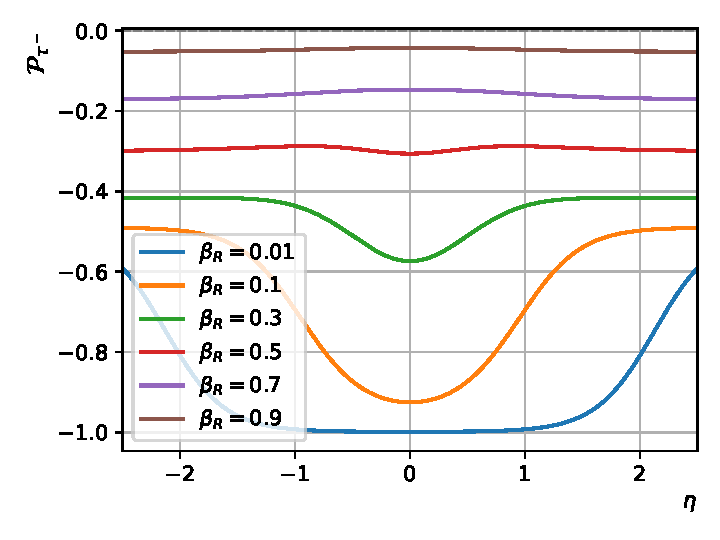
\includegraphics[width=.9\linewidth]{Images/P_vlQ_tau_minus_vs_eta_avg.pdf}
    \captionof{figure}{The average polarization asymmetry $\mathcal{P}_{\tau^-}^{\text{avg}}$ of the $\tau$ lepton as a function of its pseudorapidity $\eta$ for different values of the $\beta_R^{b\tau}$ parameter.}\label{fig:polarization_asymmetry_avg}
\end{center}

\section{A simplified model for a $\zb'_{B-L}$ boson}

Hypothetical heavy neutral bosons, such as the $Z'$ boson, are a common feature in many BSM models. They arise from extended gauge symmetries and can couple to fermions in ways that differ from the SM $Z$ boson. Assuming a $U(1)_{B-L}$ extension of the SM gauge group, the $Z'$ boson can couple to fermions through a gauge interaction that is proportional to their brayon minus lepton number ($B-L$). This coupling can lead to new interactions and processes that are not present in the SM, such as flavor-changing neutral currents or enhanced production of certain final states depending on the symmetry breaking pattern and the mass of the $Z'$ boson. Additionally, we could consider textures in the flavor space of the $Z'$ couplings, which can lead to preferential couplings to specific generations of fermions and to avoid large flavor-changing neutral currents (FCNCs) we assume that they are diagonal in the flavor space.

Accordingly, we assume the $\zb'$ only couples to third-generation fermions. Our simplified model is thus extended by:
\begin{eqnarray}
    \label{eq:BasicLagrangianZp}
        \mathcal{L}_{Z^{\prime}}&= & -\frac{1}{4} Z_{\mu \nu}^{\prime} Z^{\prime \mu \nu}+\frac{1}{2} M_{Z^{\prime}}^2 Z_\mu^{\prime} Z^{\prime \mu} \nonumber \\
        && + \frac{g_{Z^{\prime}}}{2 \sqrt{6}} Z^{\prime \mu} (\zeta_q \bar{Q}_3 \gamma_\mu Q_3 -3 \zeta_{\ell} \bar{L}_3 \gamma_\mu L_3 \\
        && \qquad +\zeta_t \bar{t}_R \gamma_\mu t_R  +\zeta_b \bar{b}_R \gamma_\mu b_R-3 \zeta_\tau \bar{\tau}_R \gamma_\mu \tau_R)
\end{eqnarray}
where the constants $M_{\zb^{\prime}}$, $g_{Z^{\prime}}$, $\zeta_q $, $\zeta_t $, $\zeta_b$, $\zeta_{\ell}$, $\zeta_\tau$, are model dependent.

Unlike the $U_1$ vector leptoquark, the polarization of the $\tau$ lepton implies the opposite polarization of the anti-$\tau$ lepton, due they are produced in the same chiral line. To differentiate the contributions of each $\zeta$ parameter, we have calculated the amplitudes for the different initial and final state polarizations, which are given by:
\begin{align}
    \abs{\mathcal{M}(b_L \bar b_R \to \tau^+_R \tau^-_L)}^2 &\propto g_{Z'}^4 \zeta_\ell^2 \zeta_q^2 \left(1+\tanh \eta\right)^2, \\
    \abs{\mathcal{M}(b_R \bar b_L \to \tau^+_R \tau^-_L)}^2 &\propto g_{Z'}^4 \zeta_\ell^2 \zeta_b^2 \left(1-\tanh \eta\right)^2, \\
    \abs{\mathcal{M}(b_L \bar b_R \to \tau^+_L \tau^-_R)}^2 &\propto g_{Z'}^4 \zeta_\tau^2 \zeta_q^2 \left(1-\tanh \eta\right)^2, \\
    \abs{\mathcal{M}(b_R \bar b_L \to \tau^+_L \tau^-_R)}^2 &\propto g_{Z'}^4 \zeta_\tau^2 \zeta_b^2 \left(1+\tanh \eta\right)^2.
\end{align}
Figure~\ref{fig:cross_section_zprime} shows the integrated production cross sections at $\sqrt{s} = 13.0\; \si{\tera\electronvolt}$ for a fixed set of couplings $g_{Z'} = 1.0$, $\zeta_\ell = 1.0$, $\zeta_q = 1.0$, $\zeta_b = 0.8$, and $\zeta_\tau = 0.6$. The cross section is sensitive to the choice of the couplings, and thus can be used to probe the underlying BSM model.
\begin{center}
    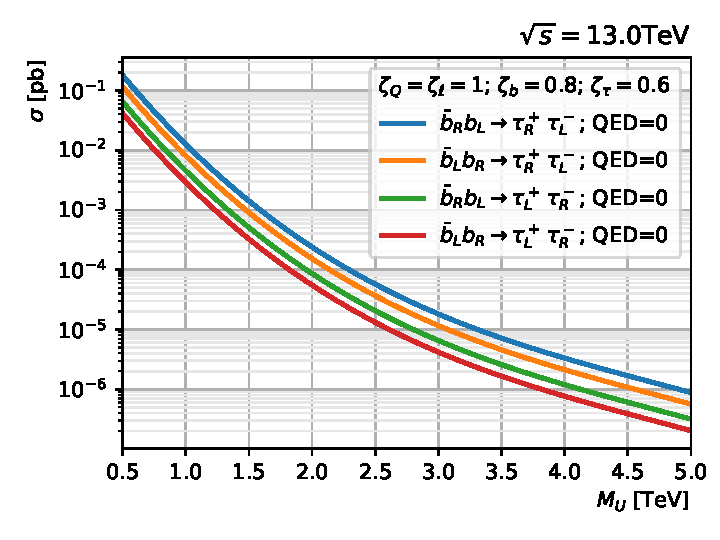
\includegraphics[width=.9\linewidth]{Images/Zprime_Cross_Section.pdf}
    \captionof{figure}{Cross section for $\zb'$ production decaying to $\tau^+\tau^-$ final states, showing different $\tau$ polarization configurations as a function of $\zb'$ mass at $\sqrt{s}=13.0 \si{\tera\electronvolt}$. The couplings are fixed to $g_{Z'} = 1.0$, $\zeta_\ell = 1.0$, $\zeta_q = 1.0$, $\zeta_b = 0.8$, and $\zeta_\tau = 0.6$.}\label{fig:cross_section_zprime}
\end{center}
The polarization asymmetry $\mathcal{P}_{\tau^-}$ of the $\tau$ lepton can be defined in a similar way as for the $U_1$ vector leptoquark, but now it is sensitive to the different couplings $\zeta_\ell$, $\zeta_q$, $\zeta_b$, and $\zeta_\tau$. The polarization asymmetry is given by:
\begin{align}
    \mathcal{P}_{\tau^-} &= \frac{\abs{\mathcal{M}_R}^2 - \abs{\mathcal{M}_L}^2}{\abs{\mathcal{M}_R}^2 + \abs{\mathcal{M}_L}^2} 
    \\&= \frac{(1+\tanh \eta)^2\left(\zeta_\tau^2 \zeta_b^2- \zeta_\ell^2 \zeta_q^2\right)
    +(1-\tanh \eta)^2\left(\zeta_\tau^2 \zeta_q^2 - \zeta_\ell^2 \zeta_b^2\right)}{
        (1+\tanh \eta)^2\left(\zeta_\tau^2 \zeta_b^2+ \zeta_\ell^2 \zeta_q^2\right)
        +(1-\tanh \eta)^2\left(\zeta_\tau^2 \zeta_q^2 + \zeta_\ell^2 \zeta_b^2\right)
    },
\end{align}
where we have defined the right-handed and left-handed contributions as
\begin{align}
    \abs{\mathcal{M}_R}^2 &= \frac{1}{2}\left(\abs{\mathcal{M}(b_R \bar b_L \to \tau^+_L \tau^-_R)}^2 + \abs{\mathcal{M}(b_L \bar b_R \to \tau^+_L \tau^-_R)}^2\right), \\
    \abs{\mathcal{M}_L}^2 &= \frac{1}{2}\left(\abs{\mathcal{M}(b_R \bar b_L \to \tau^+_R \tau^-_L)}^2 + \abs{\mathcal{M}(b_L \bar b_R \to \tau^+_R \tau^-_L)}^2\right).
\end{align}
Similarly, the polarization of $t\bar t$ observables in $Z'_{B-L}$ will depend on the couplings $\zeta_q$, $\zeta_b$, and $\zeta_t$, and can be used to measure the parameters of the underlying BSM model.

\section{Inteference between the $U_1$ and $\zb'_{B-L}$ models}

The presence of a $\zb'$ boson in $\lq$ models has been justified in various papers, for example, in~\parencite{Baker:2019sli}. The argument is that minimal extensions of the SM which include a massive gauge $U_1$ LQ, uses the gauge group $SU(4)\times SU(3)^{\prime}\times SU(2)_L \times U(1)_{T_R^3}$. Such an extension implies the presence of an additional massive boson, $\zb^{\prime}$, and a color-octet vector, $G'$, arising from the spontaneous symmetry breaking into the SM. Naively, the LQs are associated to the breaking of $SU(4)\to SU(3)_{[4]}\times U(1)_{B-L}$, the $G'$ arises from $SU(3)_{[4]}\times SU(3)'\to SU(3)_c$, and the $Z'$ comes from the breaking of $U(1)_{B-L}\times U(1)_{T_R^3}\to U(1)_Y$. Notice that the specific pattern of breaking, and the relations between the masses and couplings, are connected to the specific scalar potential used.  The $\zb'$ in particular can play an important role in the projected $\lq$ discovery reach, as it can participate in $\mathrm{p}\,\mathrm{p}\to\tau\tau$ production by s-channel exchange, both resonantly and as a virtual mediator. To study the effect of a $\zb'$ on the $\mathrm{p}\,\mathrm{p}\to\tau\tau$ production cross-sections and kinematics, we extend our benchmark Lagrangian in Eq.~(\ref{eq:BasicLagrangian}) with further non-renormalizable terms involving the $\zb'$ boson according to~\eqref{eq:BasicLagrangianZp}.

We study two extreme cases for the $\zb'$ mass, following~\parencite{GINO_PhysRevD.102.115015}, namely $M_{\zb'} = \sqrt{\tfrac{1}{2}}M_U<M_U$ and $M_{\zb'} = \sqrt{\tfrac{3}{2}}M_U>M_U$. We also assume the $\lq$ and $\zb'$ are uniquely coupled to left-handed currents, i.e. $\zeta_q=\zeta_\ell= 1$ and $\zeta_t=\zeta_b=\zeta_\tau=0$. With these definitions, Figure~\ref{fig:xsinterference} shows the effect of the $\zb'$ on the $\tau\tau$ production cross-section, considering $g_U = 1$, $\beta_R=0$, and different $g_{\zb^{\prime}}$ couplings. On the top panel, the cross-sections corresponding to the cases where $M_{\zb'} = \sqrt{\tfrac{1}{2}}M_U$ are shown. As expected, the $\tau\tau$ production cross-section for the inclusive case (i.e., $g_{\zb'} \neq 0$) is larger than that for the $\lq$-only non-res process ($g_{\zb'} = 0$, depicted in blue). This effect increases with $g_{\zb'}$ and, within the evaluated values, can exceed the $\lq$-only cross-section by up to two orders of magnitude. In contrast, a more intricate behaviour can be seen in the bottom panel of Figure~\ref{fig:xsinterference}, which corresponds to $M_{\zb'} = \sqrt{\tfrac{3}{2}}M_U$. Here, for low values of $M_U$, a similar increase in the cross-section is observed. However, for higher values of $M_U$, the inclusive $\mathrm{p}\,\mathrm{p}\to\tau\tau$ cross-section is smaller than the $\lq$-only $\tau\tau$ cross-section. This behaviour suggests the presence of a dominant destructive interference at high masses, leaving its imprint on the results.
\begin{figure}[]
\centering
    \begin{subfigure}[b]{.48\linewidth}
    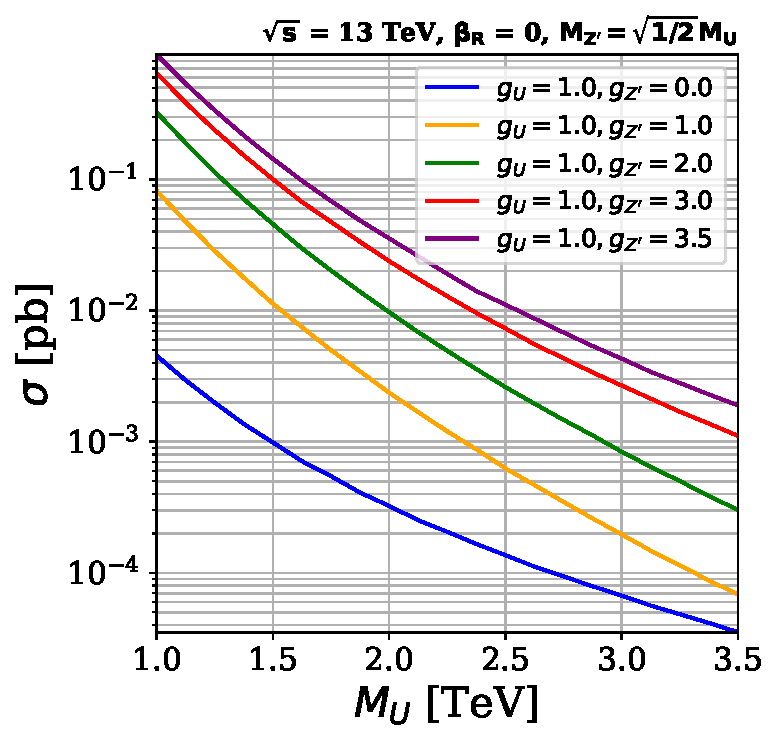
\includegraphics[width=\linewidth]{Images/XS_gu_gzp_lower_limit_woRHC.pdf}
    \end{subfigure}
    \begin{subfigure}[b]{.48\linewidth}
    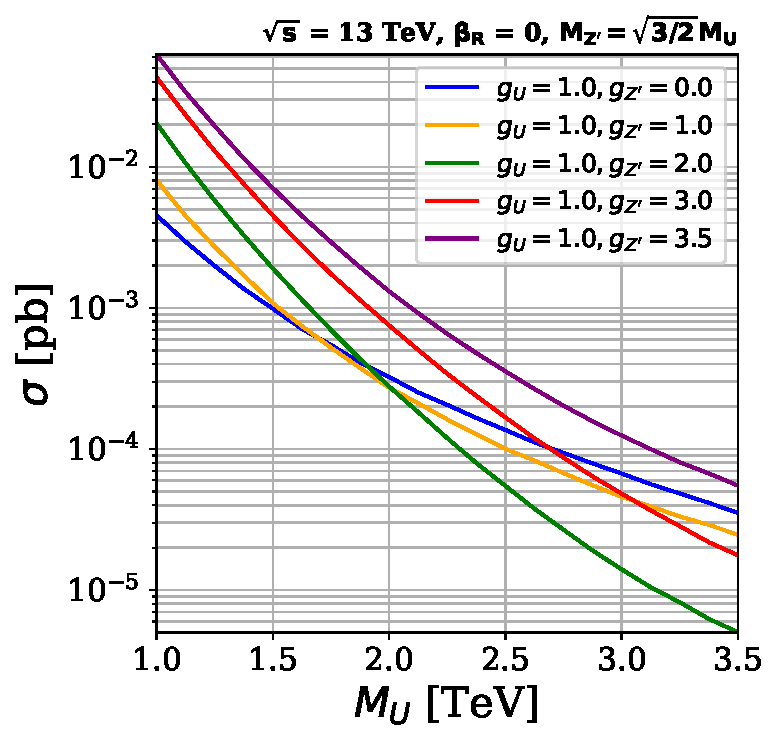
\includegraphics[width=\linewidth]{Images/XS_gu_gzp_upper_limit_woRHC.pdf}
    \end{subfigure}
    \caption{$\tau \tau$ cross-section as a function of the $\lq$ mass for different values of $g_U$ and $g_{\zb^{\prime}}$. The estimates are performed at $\sqrt s=13 \tev$, $\beta_R=0$,  $M_{\zb^{\prime}} = \sqrt{1/2} M_{U}$ (left), and $M_{\zb^{\prime}} = \sqrt{3/2} M_{U}$ (right).}
\label{fig:xsinterference}
\end{figure}

\begin{figure}[]
\centering
    \begin{subfigure}[b]{.48\linewidth}
    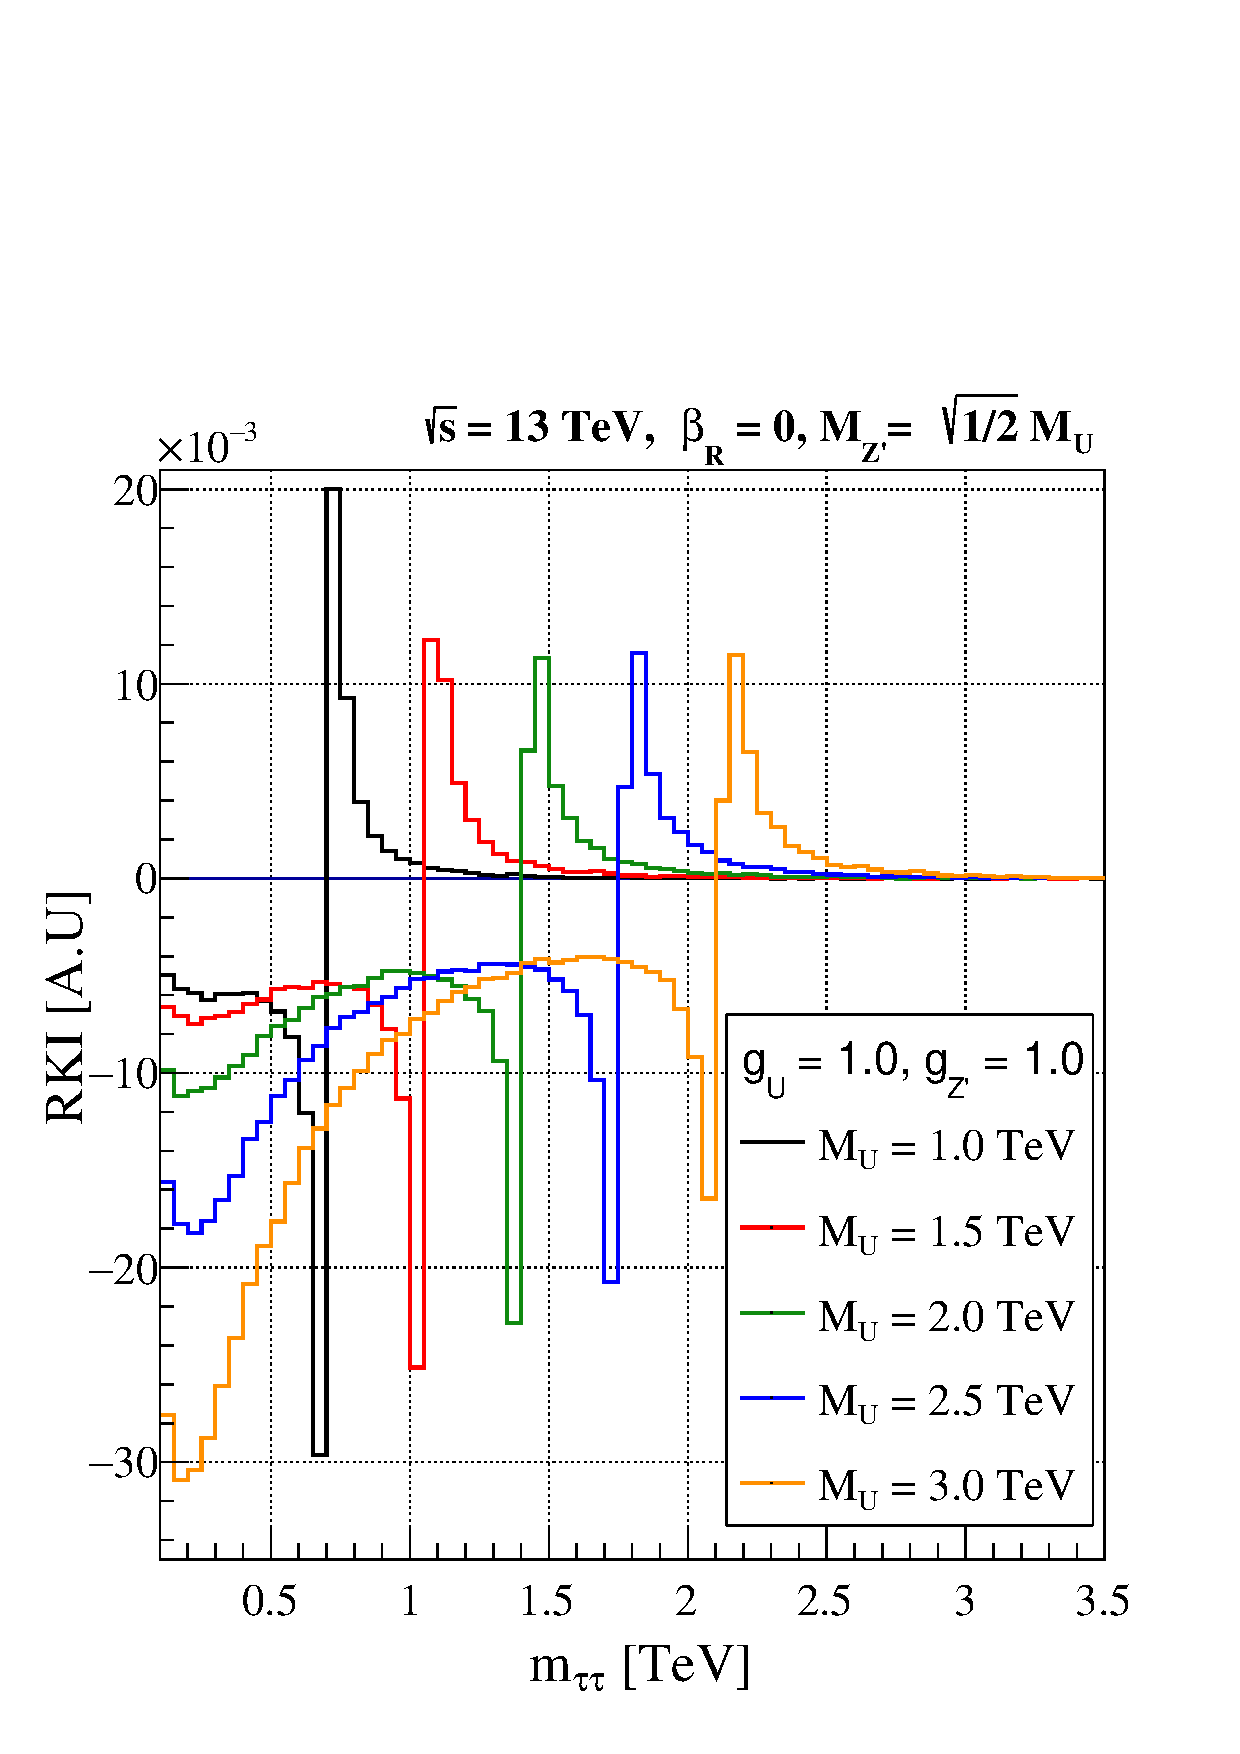
\includegraphics[width=\linewidth]{Images/Kinematic_Interference_gu_1.0_gzp_1.0_zp_lower_limit_woRHC.pdf}
    \end{subfigure}
    \begin{subfigure}[b]{.48\linewidth}
    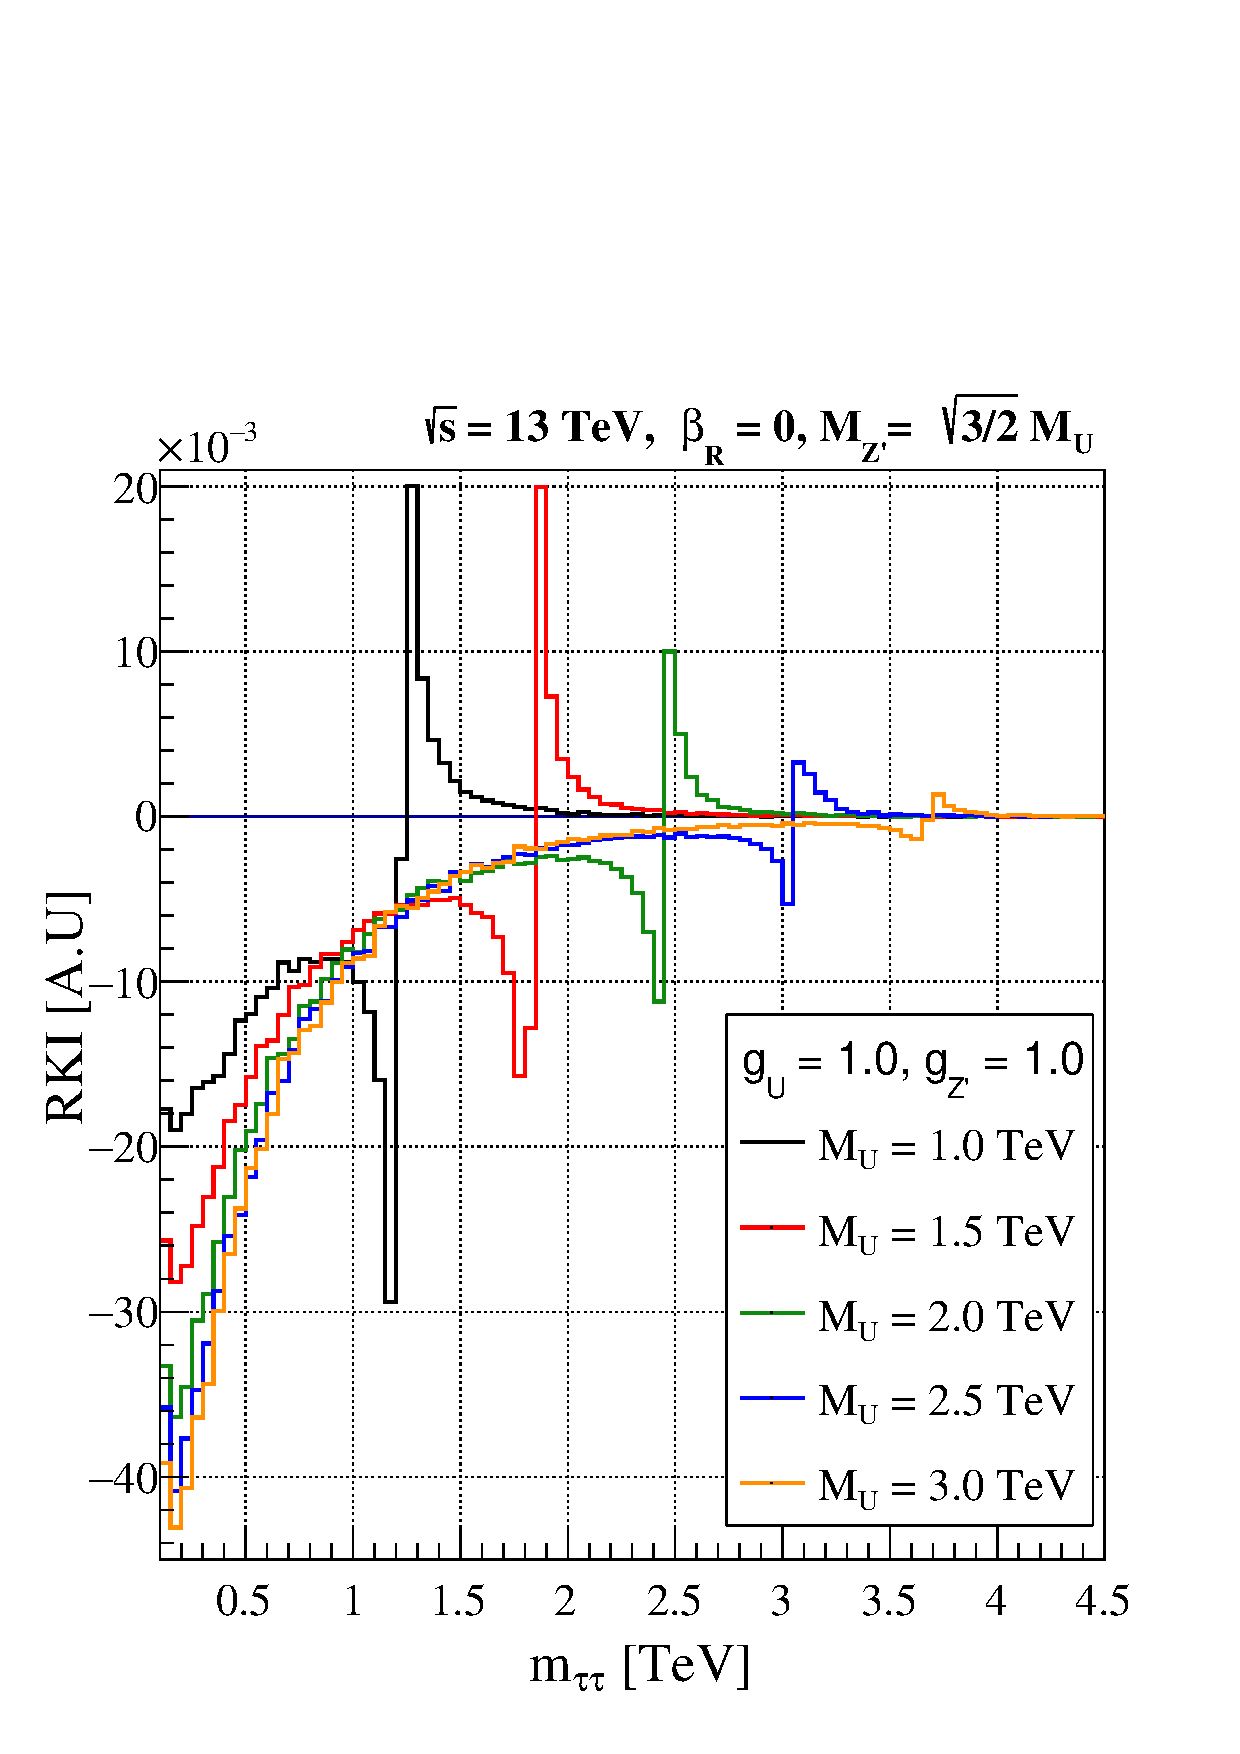
\includegraphics[width=\linewidth]{Images/Kinematic_Interference_gu_1.0_gzp_1.0_zp_upper_limit_woRHC.pdf}
    \end{subfigure}
    \caption{The relative kinematic interference (RKI), as a function of the reconstructed mass of two taus, for different $\lq$ masses. The studies are performed assuming $\sqrt s=13 \tev$, $\beta_R=0$, $g_U = 1.0$, $g_{\zb^{\prime}} =1.0$, $M_{\zb^{\prime}} = \sqrt{1/2} M_{U}$ (left), and $M_{\zb^{\prime}} = \sqrt{3/2} M_{U}$ (right).
    }    
\label{fig:interference}
\end{figure}
In order to further illustrate the effect, Figure~\ref{fig:interference} shows the relative kinematic interference ($\mathrm{RKI}$) as a function of the reconstructed invariant mass $m_{\tau\tau}$, for $g_{\zb^{\prime}} = 1$ and varying values of $M_U$. The RKI parameter is defined as
\begin{equation}
    \mathrm{RKI}(m_{\tau\tau})=\frac{1}{\sigma_{\lq+\zb'}}\left[\frac{d\sigma_{\lq+\zb'}}{dm_{\tau\tau}}-\left(\frac{d\sigma_{\lq}}{dm_{\tau\tau}}+\frac{d\sigma_{\zb'}}{dm_{\tau\tau}}\right)\right],
\end{equation}
where $\sigma_{X}$ is the production cross-section arising due to contributions from $X$ particles. For example, $\sigma_{\lq+\zb'}$ represents the inclusive cross-section where both virtual $\lq$ and s-channel $\zb'$ exchange contribute. For both cases, we can observe the presence of deep valleys in the RKI curves when $m_{\tau\tau}\to0$, indicating destructive interference between the $\lq$ and the $\zb'$ contributions. This interference generates a suppression of the differential cross-section for lower values of $m_{\tau\tau}$ and, therefore, in the integrated cross-section. 
 
%The observed interference effects are consistent with detailed studies on resonant and non-res $\mathrm{p}\,\mathrm{p}\to\tq \bar{\tq}$ production, performed in reference~\parencite{Djouadi:2019cbm}.


